% DO NOT COMPILE THIS FILE DIRECTLY!
% This is included by the other .tex files.

\begin{frame}[t,plain]
\titlepage
\end{frame}

\begin{frame}[t]{Contents of this presentation}
\begin{itemize}
	\item Progress
	\item Revised backlog
	\item Second sprint description 
	\item Final sprint 
	\item Feedback
\end{itemize}
\end{frame}

\begin{frame}[t]{Progress}
\framesubtitle{Estimated deliverable}

\vspace{1 em}
System that can, given an input and a method, apply the method to the input and return a set of recommended documents. Also, it can apply it to all documents in the input and return an automated evaluation metric, this can be used to compare the methods. 

\vspace{1em}
Additionally, a document/notebook is provided which shortly describes the implemented methods and some documentation about exploration of other methods. 
\end{frame}

\begin{frame}[t]{Progress}

\begin{itemize}
	\item 

	\item Shift to more network based approach

	\item Deciding when to stop returning documents is hard.	
\end{itemize}
\end{frame}


\begin{frame}[t]{Product Backlog}
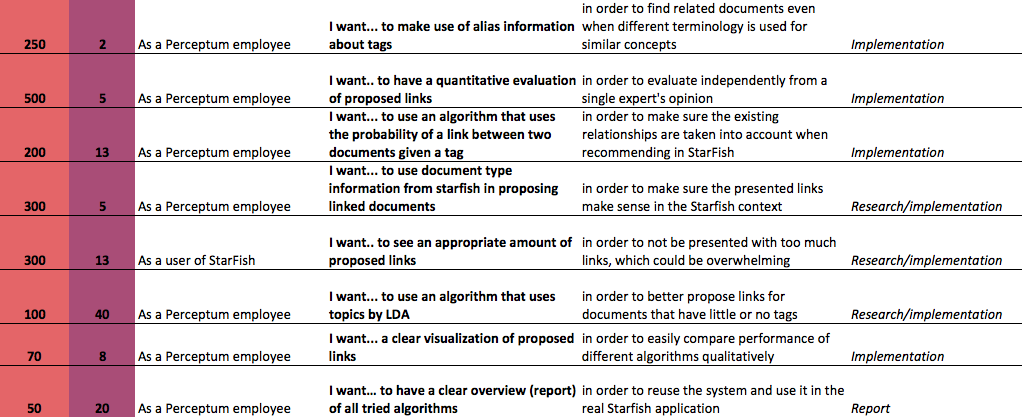
\includegraphics[width=\linewidth]{backlog2}
\end{frame}

\begin{frame}[t]{Definition of Done (recap)}
\framesubtitle{Product Backlog}

\begin{itemize}
	\item  The code is written OOP, and the classes that act correctly within the application framework
	\item The code is documented in a notebook containing examples of usage, test results and description of design choices 
	\item The code is well tested both individually as within the application flow (this may be done manually – no automated tests)
\end{itemize}
\end{frame}

\begin{frame}[t]{Sprint 2}

\end{frame}

\begin{frame}[t]{Sprint 3}

\end{frame}

\begin{frame}[t]{Feedback}
We would love to hear what you think about our planning! Are there any suggestions or questions?
\end{frame}
